\chapter{Implementation}
\label{chp:imp}
This Chapter will explain one way to implement a system based on TinyOS like the one described in Chapter \ref{chp:apr}. First, it will give a general overview of the system's structure. Then the individual parts of the system are explained in more detail.    

\section{General Structure}
\label{chp:imp_general}
The system is divided into two main components. The base station, which stores and processes the data, and the nodes, that collect the data. Both parts of the system need their own hardware and software to complete their tasks.  

\begin{figure}[htbp]
	\centering
    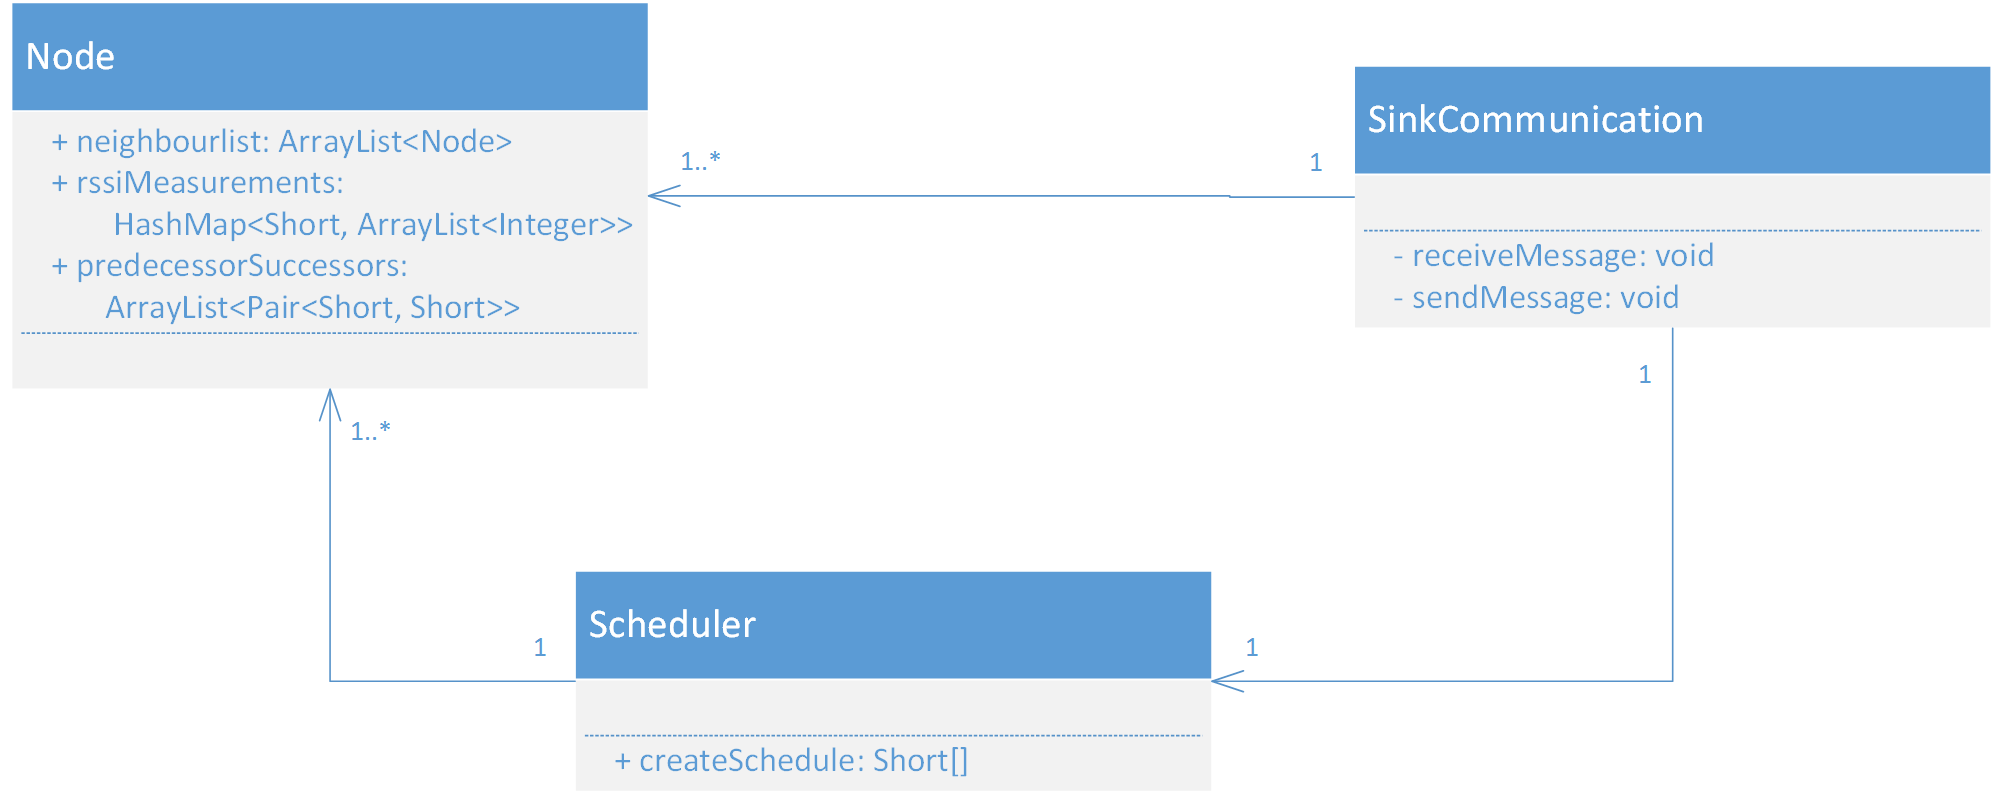
\includegraphics[scale=0.7]{content/images/BaseStation/Klassendiagram}
   	\caption{General structure and functionality of the base station.}
    \label{fig:bsKlassen}
\end{figure}

The base station can be a computer running a Java application connected to the sink via a USB-Cable. In Figure \ref{fig:bsKlassen}, you can see the general structure of the Java application with its classes and their basic functionality. First, there is the $SinkCommunication$ class that handles the communication with the sink. It is responsible for receiving and processing messages and for sending messages to the sink. Then there is the $Node$ class which stores all the information about one node. It stores the neighbours of the node, the measurements a node made and its predecessors and successors in the schedule. The last class is the $Scheduler$ that is responsible of creating a schedule based on the nodes data.  

\begin{figure}[htbp]
	\centering
    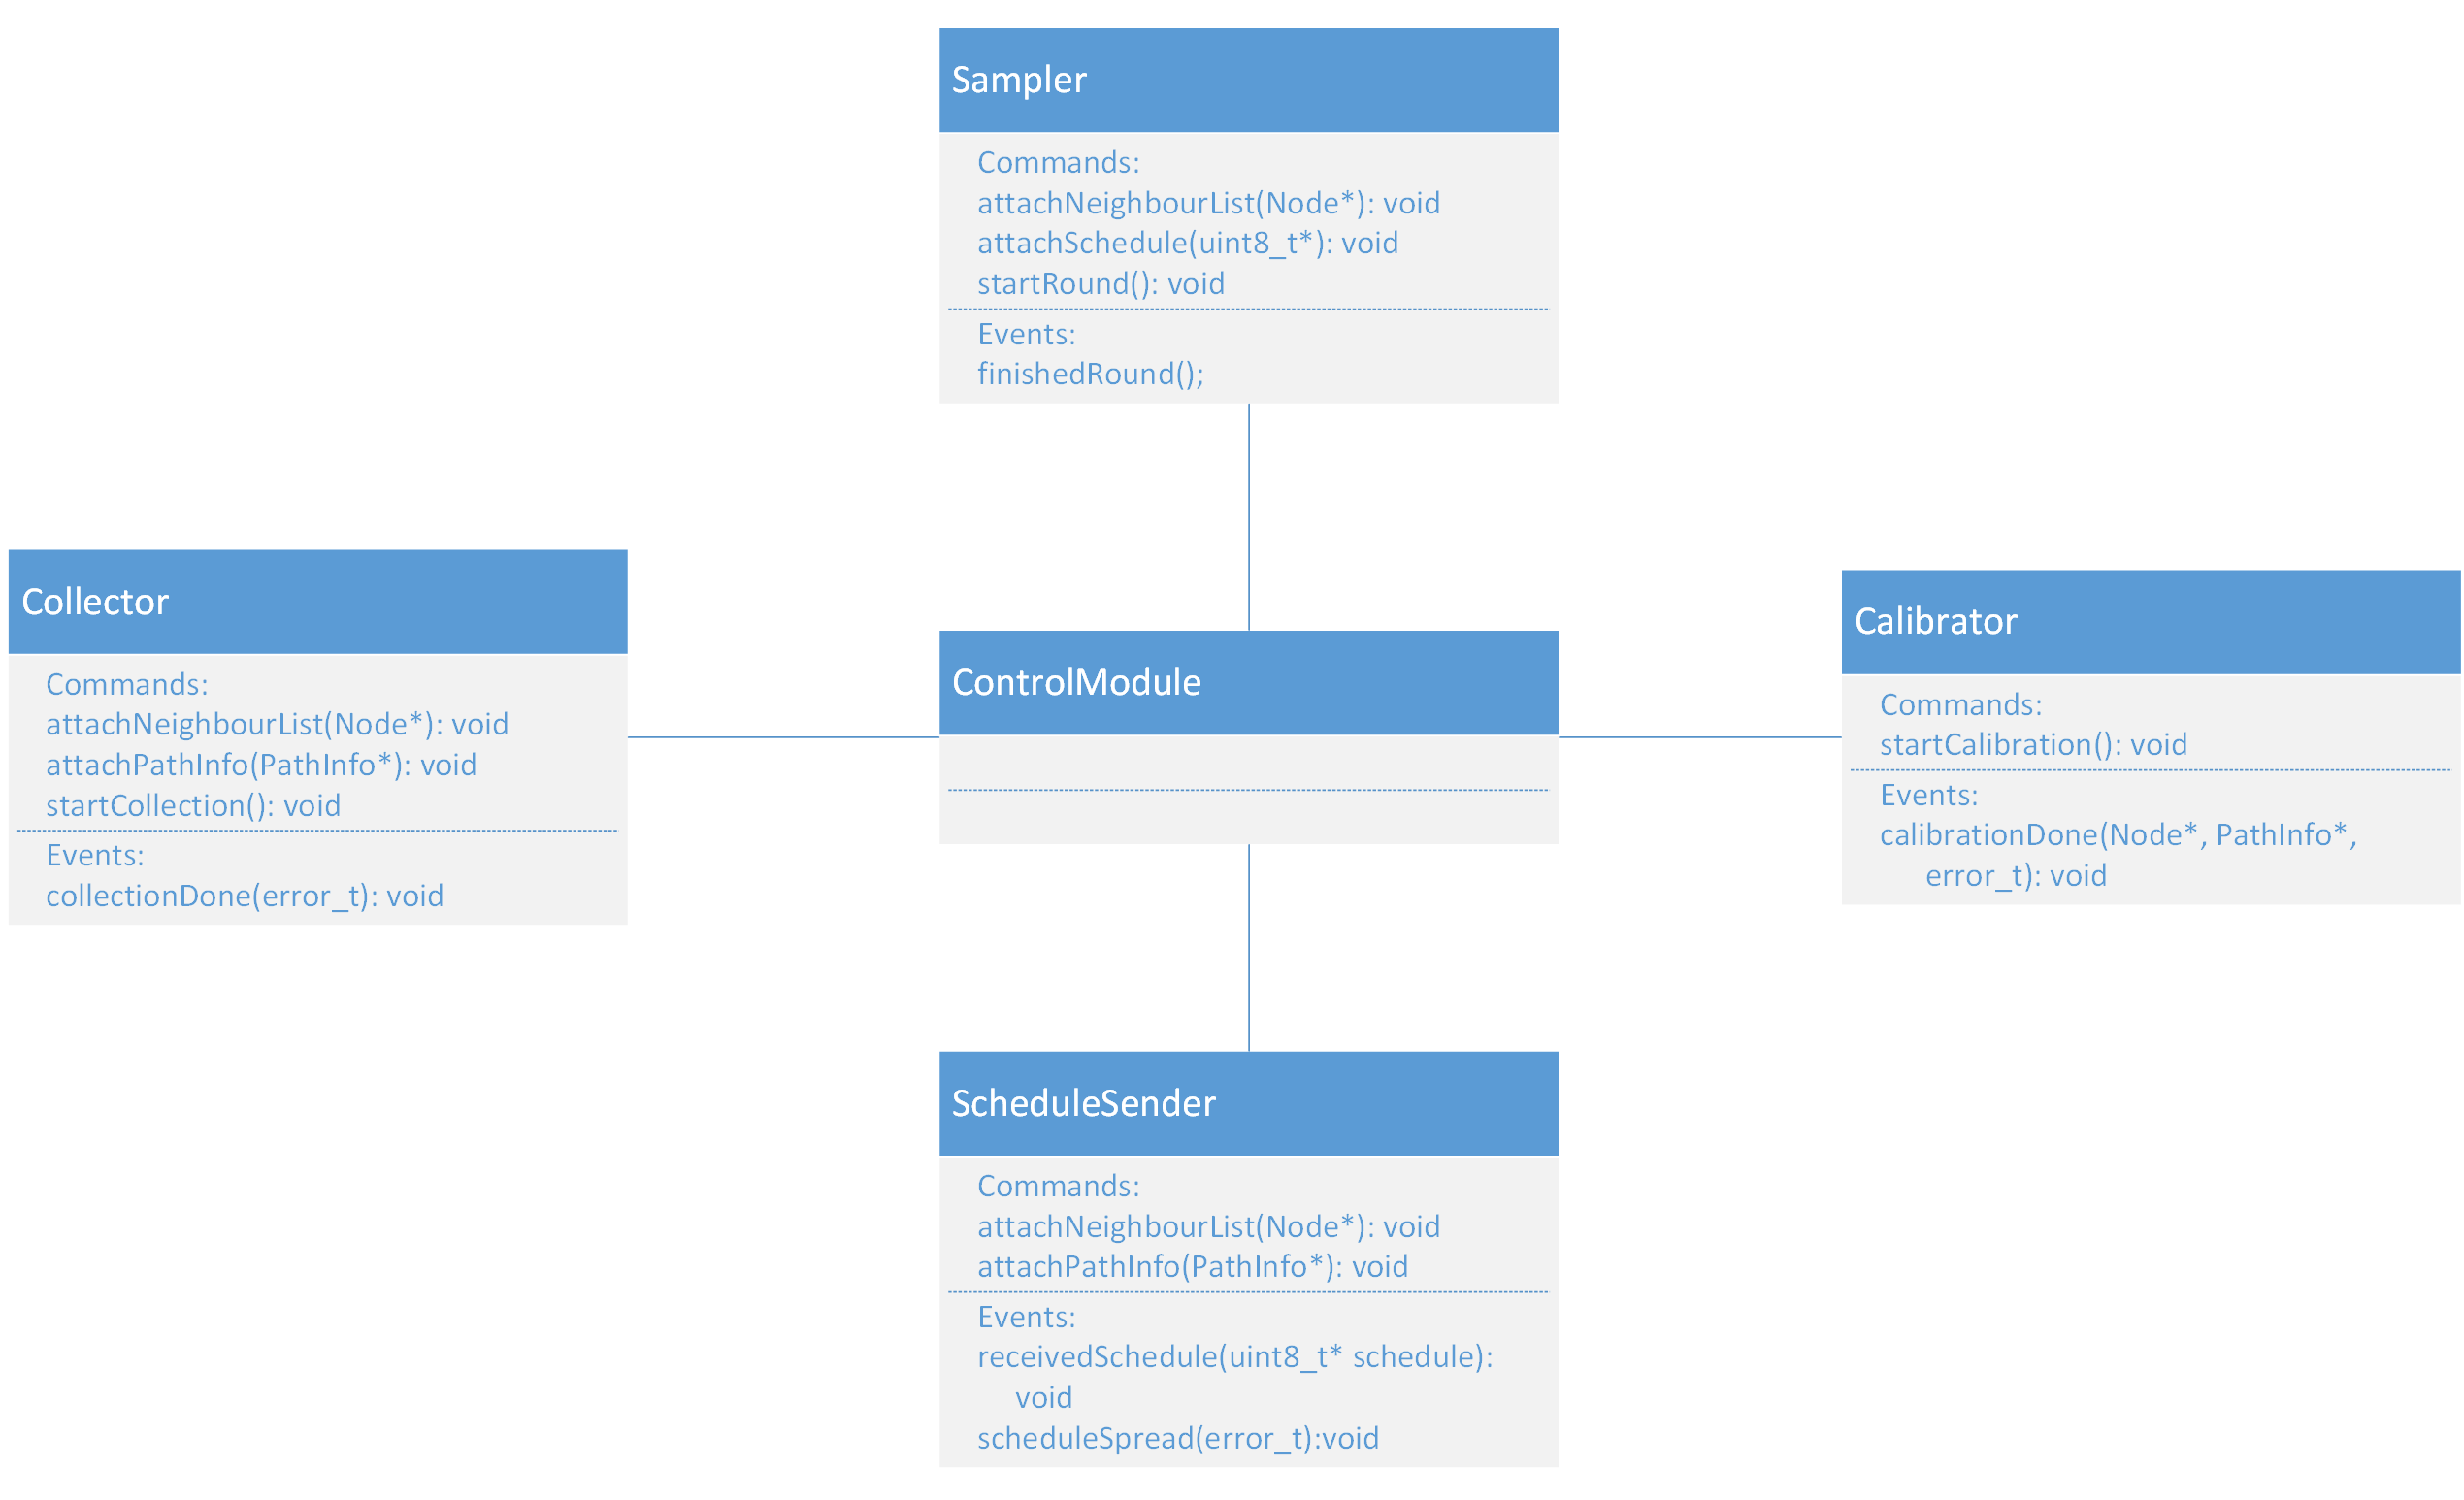
\includegraphics[scale=0.6]{content/images/Motes/GeneralStructure}
   	\caption{The interfaces each component provides. The $ControlModule$ does only use all the other interfaces and does not provide one itself.}
    \label{fig:moteStructure}
\end{figure}

As nodes the TelosB motes described in Chapter \ref{chp:TelosB} can be used. The application running on the nodes can then be written in nesC for TinyOS. Since the application running on the motes has multiple independent tasks, it makes sense to create one component for each task. In Figure \ref{fig:moteStructure} the suggested structure is displayed, containing the components $Control$, $Calibrator$, $Sampler$, $ScheduleSender$ and $Collector$ represented by their provided interfaces. 

The $Control$ component connects all the other components and makes sure the information the other components provide get delivered correctly to the component needing that information. Therefore it does not need an interface to provide functionality.     
The $Calibrator$ component is responsible for the calibration of the network. It has the $startCalibration$ command to start the calibration and the $calibrationDone$ event that gets signaled when the calibration is done and provides the gathered information. The $Collector$ component covers the data collection. This component needs to know the neighbours and the information about the node's parent and children. Therefore the interface of the component provides the two commands $attachNeighbourList$ and $attachPathInfo$ to attach this information to the component. The $Control$ component can then simply attach the information to the $Collector$ when the $calibrationDone$ event triggers. Moreover, the $Collector$ component needs the event $collectionDone$ to signal when the collection is done. To spread the schedule inside the network, the application provides the $ScheduleSender$ component. It also needs the information about the neighbours and the parent and children of the node and therefore has the same commands as the $Collector$ to attach this information to it. It does not necessarily need a command to start the spreading since it can directly react when the node receives a schedule message from the base station. Last, the component has two events $receivedSchedule$ and $scheduleSpread$. The component signals the $receivedSchedule$ event when the node received the schedule and provides the schedule. When the schedule is spread, the sink signals the $scheduleSpread$ event. The last component is the $Sampler$. It needs the neighbour list and the schedule and therefore has the commands $attachNodeList$ and $attachSchedule$ to provide these to the component. Moreover it has the $startRound$ command to start one round of the schedule and the $finishedRound$ event that the component signals when this round is finished. Figure \ref{fig:commandEvents} represents a possible sequence of the commands and events.

\begin{figure}[btp]
	\centering
    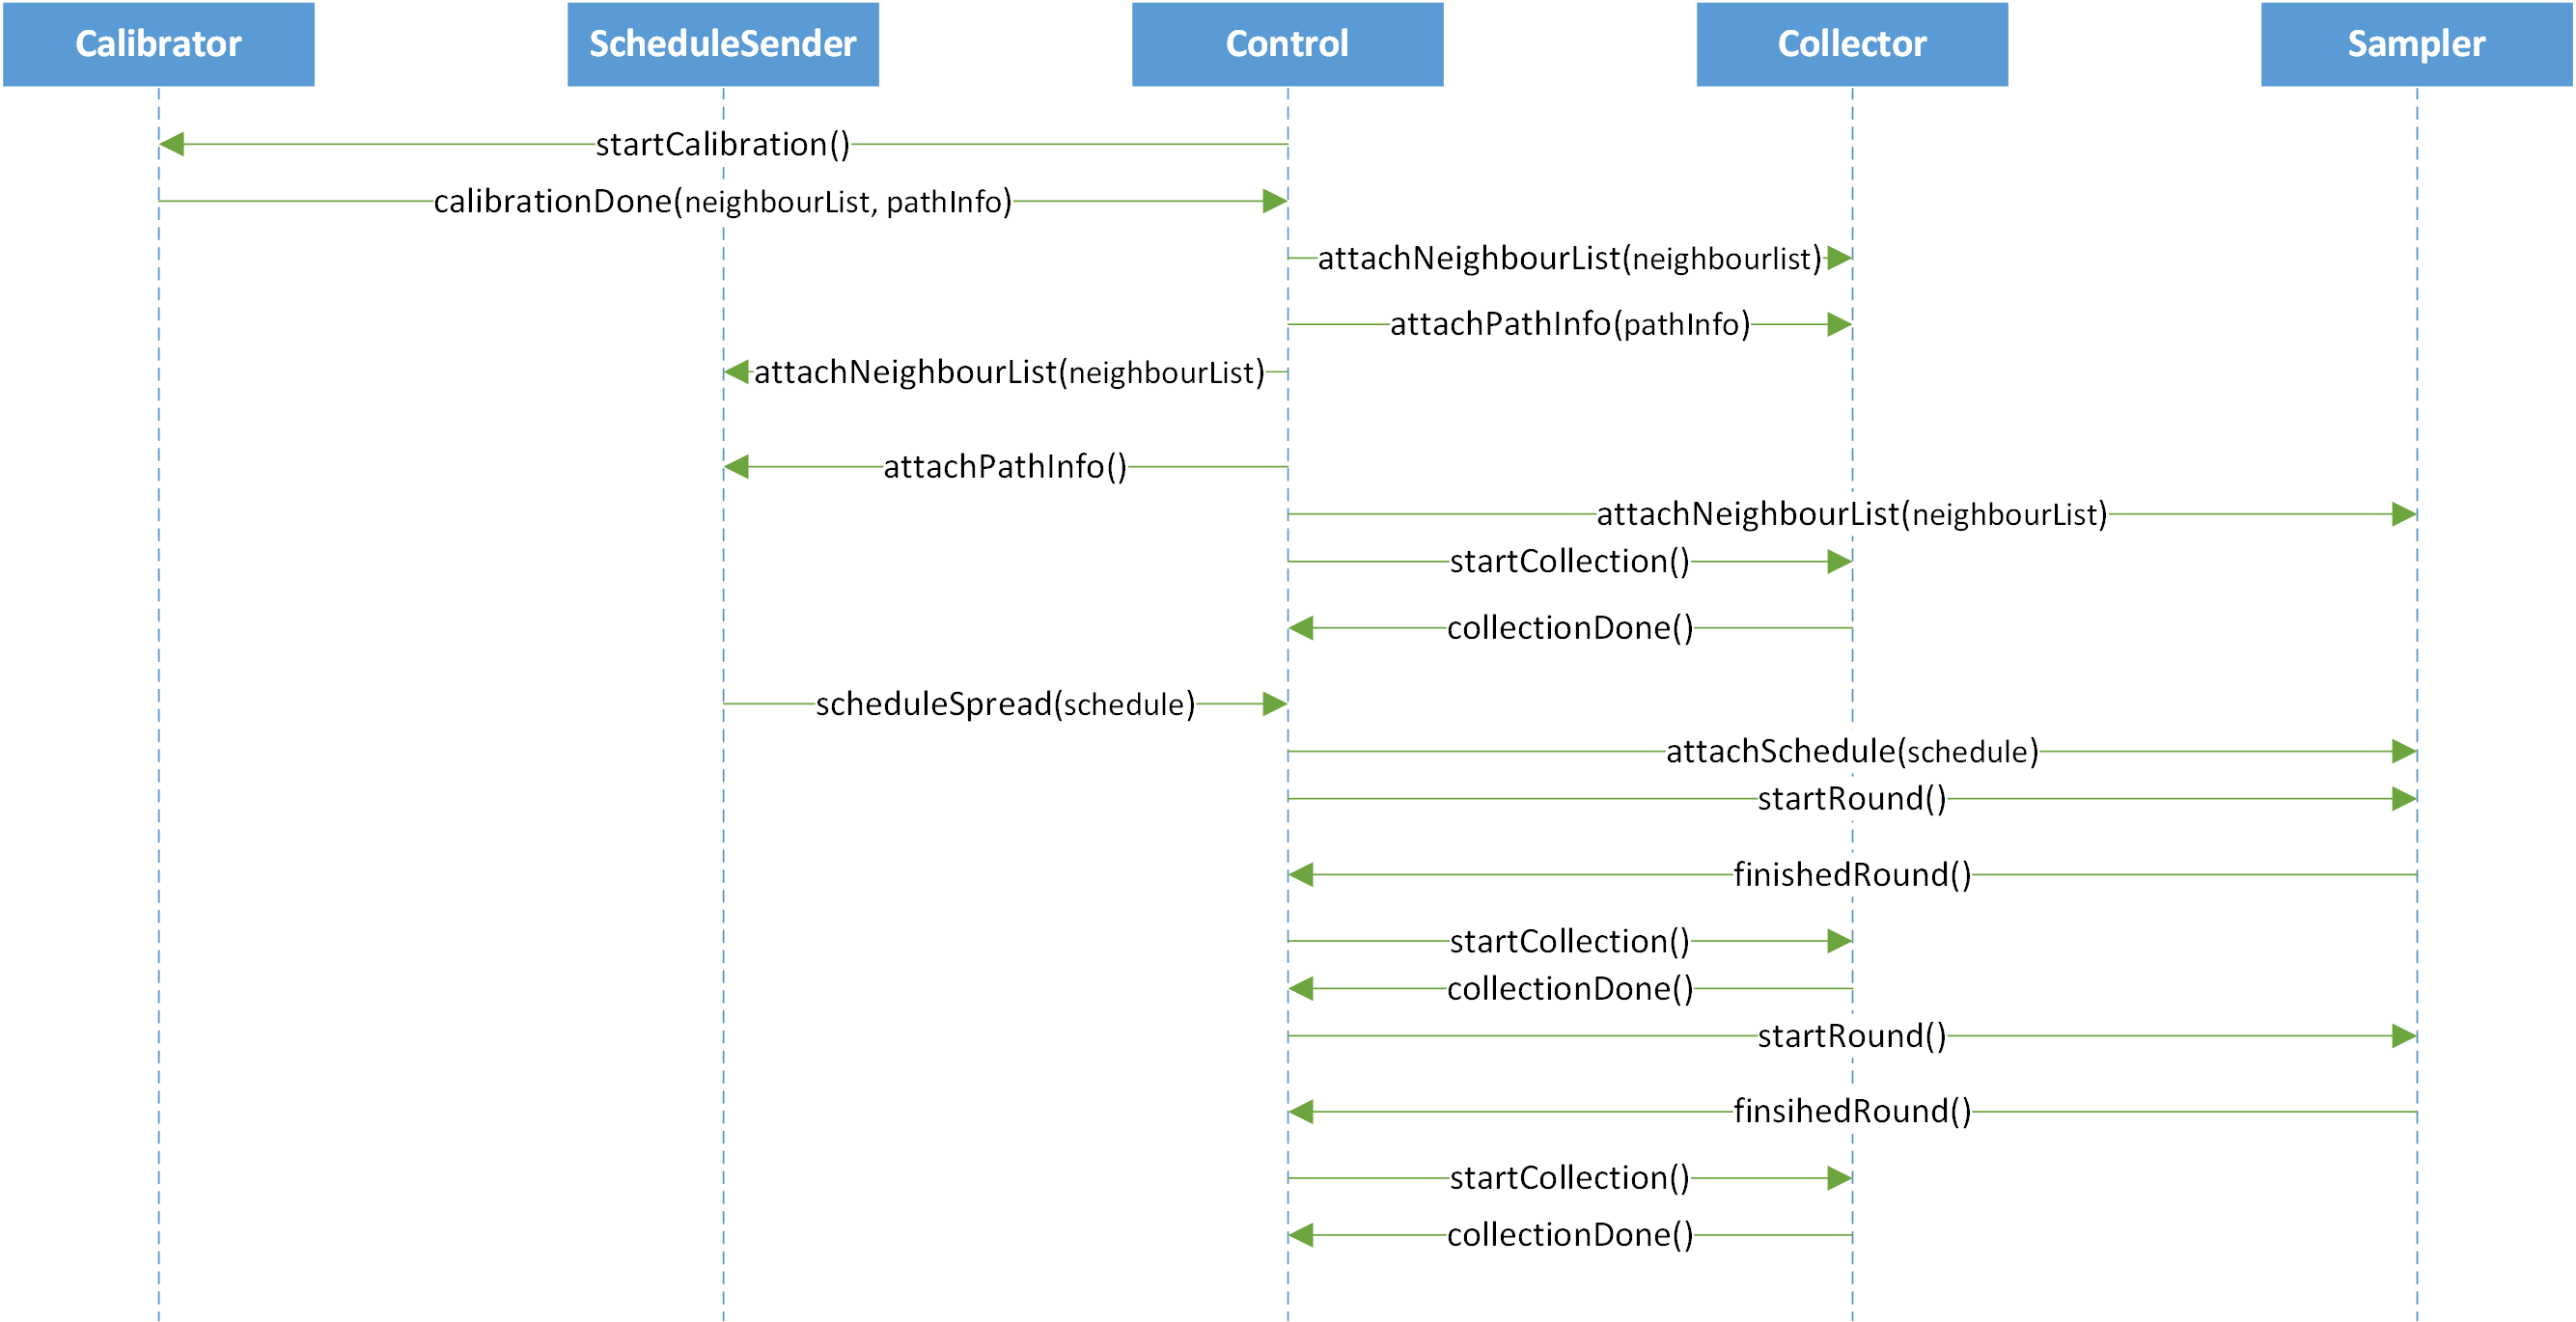
\includegraphics[scale=0.55]{content/images/Processes/ComandsEvents}
   	\caption{The order of commands and events of the sink from the start of the application until the sampling.}
    \label{fig:commandEvents}
\end{figure}

\section{Receiving and Storing Information at the Base Station}
\label{chp:imp_baseStation}
To receive and send messages from the sink, it is possible to make use of the TinyOS Java libraries. These provide the necessary tools to connect the application to the sink via a serial forwarder. To synchronize the message types sent by the motes and the Java application, TinyOS provides the possibility to generate message classes directly from the nesC message structures. The Java application needs to know two different messages. One that contains the information collected by a node and one that contains the information about the schedule. The application now needs to implement message listener for both types of messages so it is able to receive and react to each message individually.

To store information about all the nodes, the Java application needs to implement a hash map containing one $Node$ object for every node inside the network with its ID as the key. This makes it easy to access the information of each individual $Node$ object. To store the information about a node's neighbours, the $Node$ class implements a list containing references to $Node$ objects representing the neighbours of the node. To store the RSS measurements of a node, the $Node$ class implements a hash map containing lists. Again the key values of the hash map are node IDs. The lists inside the hash map contain all the measurements from the node corresponding to the key. 

Now whenever the Java application receives a message containing measurements of a node, it gets the corresponding node object from the hash map containing all the nodes. Then it updates the neighbour list of the node and saves the measurements inside the measurement hash map of the node object.
\section{Calibration}
\label{chp:imp_calibration}
To calibrate the network by using the procedure explained in Chapter \ref{chp:apr_calibration}, the Calibration component needs to send messages without a specific pattern. These messages need to contain information about the path quality and the parent of the node. A possible message structure that fulfills these requirements is shown in Listing \ref{lis:callMsg}. 

\lstset{caption={Message structure for the messages containing information about the parent and the path quality of the sending node.},label={lis:callMsg}}
\begin{lstlisting}
	nx_struct CalibrationMsg {
		uint8_t parent,
		uint8_t path_quality
	}
\end{lstlisting}

To make sure that all the nodes send their messages roughly in the same time interval, a way to indicate when the calibration starts is needed. This can be achieved by one node starting its calibration phase and the sending of messages. Then when another node receives a $CalibrationMsg$ and has not started its calibration it starts its calibration. Another problem is that if all the nodes send their messages directly one after another there would be a lot of messages in the network at the same time. To reduce this, each node has a small delay between the messages it sends. To make this even more efficient, each node has a different delay between its messages. This delay can be calculated as  
\[ \Delta p = T + \mbox{ID}^2\ \%\ N\]
where $T$ is the minimal time between sends, $ID$ is the node's ID, and $N$ the number of nodes in the whole network. Now whenever a node sends a message, it can start a timer that fires after $\Delta p$ and then it can send the next message when the timer fires. Whenever a node sends a message, it includes its stored parent and path quality.  

To collect data from other nodes, each node needs a neighbour list where it can store the nodes in range and the measured values. This neighbour list can be implemented by an array of the $Node$ struct shown in Listing \ref{lis:nodeStr} with the size $N$. The structure can store the last received signal strength, if the node is in range and the parent of the node. The other fields are used for the other phases. 

Whenever a node receives a message, it first sets the $inRange$ field for that node to $true$, stores the measured received signal strength in the $last\_rssi$ field and sets the $parent$ field to the $parent$ field inside the message. 
 
\lstset{caption={Structure to store information about nodes, containing the last RSS measured, if the node is in range, the parent of the node, if the node received the data from node, if the node received the schedule from the node and the messages received from the node.},label={lis:nodeStr}}

\begin{lstlisting}
	typedef struct Node {
  		int8_t last_rssi;
  		int8_t inRange;
  		uint8_t parent;
  		int8_t receivedData;
  		int8_t receivedSchedule;
  		uint16_t msg_counter;
	}
\end{lstlisting}

The next thing for the node is to evaluate if it should use the sending node as a parent. This is done like explained in Chapter \ref{chp:apr_collection}. However, the link quality is not directly described by the RSS. Instead the RSS is mapped to a value where a high RSS represents a low value and a low RSS a high value. An example for the mapping of the RSS to the path quality is given in Table \ref{tab:mappingRSSI}. The mapped value then represents the link quality, where a lower value indicates a better path quality.

This mapping is determined by the links inside the used WSN and needs to be defined for each WSN individually. This means if there are only links with very low RSS values it makes no sense to start the mapping at a much higher RSS.

\begin{table}[htbp]
 \caption{Example mapping of RSS to a value representing the path quality.}
 \centering
 \begin{tabular}{c|c}
  RSS & Quality\\ \toprule
  -50 & 1 \\
  -70 & 2 \\
  -80 & 7 \\
  -90 & 14 \\
 \end{tabular}
 \label{tab:mappingRSSI}
\end{table}

When the link quality is mapped, it is added to the $path\_quality$ received in the message. Then the calculated value is compared to the own stored path quality of the receiving node. If the calculated value is smaller than the stored path quality, the sending node is a more suitable parent and the stored parent and path quality are adjusted accordingly.   

A node concludes its calibration phase and signals the $calibrationDone$ event after sending a defined number of messages. This number however is also determined by the network and its complexity.  

To make sure the sink does not start to collect data from the network before every other node finished its calibration, it needs to wait after sending all its messages.
When it finished waiting, it can signal the $calibrationDone$ event. The time the sink needs to wait depends on the number of nodes, the amount of messages sent in the calibration and the calculation of the break between messages.
 
\section{Collection}
\label{chp:imp_collection}
Before starting the collection, the Collection component needs the information gathered by the Calibration component. When the neighbour list and path info are attached to the component, the sink can start the collection by sending a request message like the one in Listing \ref{lis:reqMsg} to one of its children. To find a child, a node can go through its neighbour list and simply check if the $parent$ field in the $Node$ struct is set to the ID of the node. When a node receives a request message, it searches for a child of itself and forwards the request like described in Chapter \ref{chp:apr_collection}.

\lstset{caption={Structure representing a request message.},label={lis:reqMsg}}
\begin{lstlisting}
	typedef nx_struct RequestMsg {
		nx_uint8_t id;
		nx_uint8_t round;
	}
\end{lstlisting}

When the request reaches a node without any children, the node fills its measurements into the $measurements$ field of a data message like the one represented in Listing \ref{lis:dataMsg}.
Since it is possible that a node has more measurements than the maximal amount of data fitting into one message, we need the field that indicates how much data is left. If a node has more measurements, it directly fills multiple messages and sends them one after another to its parent. The receiving node buffers all the data messages until it received the message where the $dataLeft$ field is set to zero. Then it forwards all the received messages one after another. Whenever a node received the whole dataset of a node, it marks that node as done sending by simply setting the $receivedData$ field for the node to true. Note that the receiving node does not necessarily mark the node it directly received the dataset from but the source of the dataset indicated by the $from$ field inside the data messages.

\lstset{caption={Structures to send the data from a node to the sink. The NodeMsg contains the measurements from one neighbour including the ID of the neighbour and the measured RSS. Inside the DataMsg the source of the measurements, the answered request ID and how much data is left is stored.},label={lis:dataMsg}}
\begin{lstlisting}
	typedef nx_struct Measurement {
		nx_uint8_t id;
		nx_int8_t rss;
	}

	typedef nx_struct DataMsg {
		nx_uint8_t from;
		nx_uint8_t request_id;
		nx_uint8_t dataLeft;
		Measurement measurements[MAX__MSG__PAYLOAD - 3];
	}
\end{lstlisting}

A problem that needs to be addressed are message drops. Without detecting a message drop and resending the message afterwards, the collection simply stops if one message does not get received. To detect a message drop, each node receiving a message directly sends an acknowledgement to the sending node. This is required for both the request and the data message and is done before any processing of the message. If the sending node did not get an acknowledgement for a message, it resends that message. Since not only the actual message can get lost but also the acknowledgement, it can happen that a message gets retransmitted one or multiple times although the message was already received and processed at the receiving node. The processing of the same message multiple times however can create unintended behaviour, resulting in the system to stop working and/or messages still being sent after the collection is already finished and the sampling already started thus distorting the RSS measurements. 

To prevent this, each request gets an ID from the sink in ascending order and the round of the collection. Whenever a node sent its data, it increases its saved round by one and set the saved request ID to zero. When a node receives a request, it checks if the round of the request equals the saved round. If yes, it checks if the ID of the request is larger than its saved last request ID. If that is that the case, it saves the received request ID and processes the request, otherwise it discards the requests. To catch already received data messages we include the request ID the data was requested with inside the data message. When a node receives a data message, it can then check if the data is corresponding to the request the node sent. If that is the case it also checks if the $dataLeft$ field in the message is smaller than the one in the data message previously received. If that is not the case, the data inside that message was already received and the message gets thrown away. 

\section{Creating the Schedule}
The creation of the schedule happens at the base station when it received the data about the connections between nodes. The method presented in Listing \ref{lis:rooted} could be directly translated into the fitting Java code. To do so, another class for the rooted circle needs to be added to the general structure of the application. When implementing the method, it is important to take into account that links are not always bidirectional, meaning when a node 1 is in the neighbour list of another node 2 this only means that node 2 can receive data from node 1, not necessarily that node 1 also receives messages from node 2. This means the neighbour list only contains the nodes a node can receive messages from, resulting in the fact that when we choose a node from a nodes neighbour list, the chosen node can never be a successor but only a predecessor of a node. This results in the schedule being created backwards.

Moreover it is a good idea to not simply pick a random node as a predecessor from the neighbour list of a node, but the one with the highest measured RSS. This reduces message losses while running the schedule, resulting in less time needed for one round.  

To bring the schedule into a form that is readable for all the nodes, an array can be created that contains all the node IDs in the order they are expected to send messages. For the example in Figure \ref{fig:schedule} the array looks like this: 
\[ Short[]\ schedule = \{1, 2, 3, 4, 2, 6, 5, 6, 7, 8, 9, 10, 7, 1\}\]     
\section{Spreading the Schedule}
Before the spreading of the schedule can start, the $ScheduleSender$ component needs the information collected in the Calibration. When the information is attached to the ScheduleSender, the spreading of the schedule automatically starts when the base station sends a schedule message like the one in Listing \ref{lis:scheduleMsg} to the sink. The message contains the schedule array created by the base station, then the information about how much of the schedule is left and an ID to detect already received messages. When the sink receives the schedule message, it forwards it like described in Chapter \ref{chp:apr_spreadingSchedule}.

\lstset{caption={Schedule message structure.},label={lis:scheduleMsg}}
\begin{lstlisting}
	typedef nx_struct ScheduleMsg {
		nx_uint8_t msgid;	
		nx_uint8_t dataLeft;
		nx_uint8_t schedule[MAX__MSG__PAYLOAD-2];
	}
\end{lstlisting}

Whenever a node receives a message, it first checks if it already received that part of the schedule on the basis of the $dataLeft$ field. If it did not receive that schedule part yet, it copies it to the right place in its own schedule array. Then it marks the node it got the message from and forwards it like described in Chapter \ref{chp:apr_spreadingSchedule}. Last, it checks if the $dataLeft$ field inside the just forwarded schedule message equals zero. When that is the case, the component signals the $receivedSchedule$ event and provides the full schedule array to the $Control$ component.
To make it possible to receive multiple schedule parts, it is important that whenever a node sends the schedule to its parent, it needs to unmark all its marked nodes, so if necessary it can later send the next schedule part to them.

If the schedule message reaches the sink and the sink does not have any more unmarked children, it forwards the schedule to the base station and unmarks all its marked nodes. This way the base station knows that either the schedule is spread or it can send the next schedule part that then is spread the same way as the first one. If the sink sent the last part of the schedule to the base station, the sink signals the $scheduleSpread$ event to let the $Control$ component know that every node knows the schedule and the sampling can be started. 

Again we need to make sure that no messages get lost, so in this phase as well each message is directly replied by an acknowledgement message. If the sending node did not get the acknowledgement, it resends its message. To check if a message was already received, we have the $msgid$ field in the message. Whenever a node forwards the schedule, it increases this field and saves the value. Then when a node receives a message, it checks if the $msgid$ is larger than the saved one. If that is the case, it is a new message and needs to be processed. Otherwise the message gets thrown away. 
\section{Sampling}
When the schedule is spread and the sample component knows about the schedule and the neighbour list, the sampling can start. The sink starts by broadcasting a message like the one shown in Listing \ref{lis:sampleMsg}. The $receiver$ field is set to the node ID of the successor of the sink. Then all the nodes receiving the message measure the received signal strength and save it inside their neighbour lists. Then each node that received the message compares their own ID to the ID saved in the $receiver$ field of the message. If they are equal, the node evaluates the fitting successor, saves it inside a new message and then also broadcasts it. When the sink receives a message and does not have another successor, it signals the $finishedRound$ event.

To evaluate the fitting successor, the approach coming to mind would be to just go through the schedule array and search for the sending node followed by the searching node's ID. The successor then would be the node after that. Since this would require a loop, it is inefficient and unnecessarily stretches the time slot to catch message drops. Therefore it is suggested to evaluate all the predecessors and successors of a node before the sampling starts by going through the whole schedule once and save them, in the order of appearance, in a structure like the one shown in Listing \ref{lis:scheduleSaving}. Additionally, each node stores the index of the next predecessor successor pair. Then when a node is the successor, it can simply check if the predecessor at the saved index is correct and if that is the case, send the new message to the corresponding saved successor and calculate the next index as
\[ I+1 = (I + 1)\ \%\ \mbox{numberOfPS}\]      
It can happen that the predecessor at the saved index is not corresponding to the sending node. This can happen when a message drops and the node gets skipped.
In that case we have to go through all the predecessor successor pairs to find the right successor and adjust the saved index accordingly. However this is still more efficient than going through the whole schedule.

\lstset{caption={Sample message structure.},label={lis:sampleMsg}}
\begin{lstlisting}
	typedef nx_struct SampleMsg {
		nx_uint8_t receiver;
	}
\end{lstlisting} 

\lstset{caption={Structures to save the successors and predecessors.},label={lis:scheduleSaving}}
\begin{lstlisting}
	typedef struct PredecessorSuccessor {
		uint8_t predecessor;
		uint8_t successor;
	}

	typedef struct SchedulePSCollection {
		uint8_t numberOfPS;
		PredecessorSuccessor preSuc[MAX_PREDECESSORS_SUCCESSORS]; 
	}
\end{lstlisting}

To catch the message losses like explained in Chapter \ref{chp:apr_samplingDrops}, every time a node receives a message and is not the successor, it needs to run through the schedule array and calculate how many nodes sent between the sending node and the receiving node and calculate the time it needs for the schedule to reach the node. Then the node starts a timer that fires after exactly that time. Moreover the node needs to save the successor in case of the loss. The timer is reset to the new time whenever the node receives a message. When the timer fires, the node simply sends a message with the $receiver$ set as the saved successor. Since a node can appear multiple times inside the schedule, it needs to check if it needs to send another message at a later point in time. To do so, it can pretend it received its own message and calculate the time to its next send like for any other message.  